
\documentclass{beamer}
\usepackage[utf8]{inputenc}

\usetheme{Madrid}
\usecolortheme{default}
\usepackage{amsmath,amssymb,amsfonts,amsthm}
\usepackage{txfonts}
\usepackage{tkz-euclide}
\usepackage{listings}
\usepackage{adjustbox}
\usepackage{array}
\usepackage{tabularx}
\usepackage{gvv}
\usepackage{lmodern}
\usepackage{circuitikz}
\usepackage{tikz}
\usepackage{graphicx}

\setbeamertemplate{page number in head/foot}[totalframenumber]

\usepackage{tcolorbox}
\tcbuselibrary{minted,breakable,xparse,skins}



\definecolor{bg}{gray}{0.95}
\DeclareTCBListing{mintedbox}{O{}m!O{}}{%
  breakable=true,
  listing engine=minted,
  listing only,
  minted language=#2,
  minted style=default,
  minted options={%
    linenos,
    gobble=0,
    breaklines=true,
    breakafter=,,
    fontsize=\small,
    numbersep=8pt,
    #1},
  boxsep=0pt,
  left skip=0pt,
  right skip=0pt,
  left=25pt,
  right=0pt,
  top=3pt,
  bottom=3pt,
  arc=5pt,
  leftrule=0pt,
  rightrule=0pt,
  bottomrule=2pt,
  toprule=2pt,
  colback=bg,
  colframe=orange!70,
  enhanced,
  overlay={%
    \begin{tcbclipinterior}
    \fill[orange!20!white] (frame.south west) rectangle ([xshift=20pt]frame.north west);
    \end{tcbclipinterior}},
  #3,
}
\lstset{
    language=C,
    basicstyle=\ttfamily\small,
    keywordstyle=\color{blue},
    stringstyle=\color{orange},
    commentstyle=\color{green!60!black},
    numbers=left,
    numberstyle=\tiny\color{gray},
    breaklines=true,
    showstringspaces=false,
}
\begin{document}

\title 
{1.11.2}
\date{August 28,2025}


\author 
{Yoshita J - EE25BTECH11065}






\frame{\titlepage}
\begin{frame}{Question}
  Unit vector along PQ, where coordinates of P and Q respectively are \myvec{2\\1\\-1} and \myvec{4\\4\\-7} is.\\
\end{frame}



\begin{frame}{Table}
Let the coordinates of the points be $\mathbf{P}(2, 1, -1)$ and $\mathbf{Q}(4, 4, -7)$.
\begin{table}[H]    
  \centering
  

  \caption{Vectors}
  \label{Answers}
\end{table}
\end{frame}
\begin{frame}{Theoretical Solution}
To find the vector \(\mathbf{PQ}\), we subtract the matrix for P from the matrix for Q:
\begin{align}
    \mathbf{PQ} &= \mathbf{Q} - \mathbf{P} \\
    &= 
   \myvec{4\\4\\-7}
    -
    \myvec{2\\2\\-2} \\
    &= 
    \myvec{4-2\\4-1\\-7-(-1)} \\
    &= 
    \myvec{2\\3\\-6}
\end{align}

\end{frame}

\begin{frame}{Theoretical Solution}
If we represent the vector \(\mathbf{PQ}\) as a column vector \(\mathbf{a}\):
\[
\mathbf{a} = 
\myvec{2\\3\\-6}
\]
The norm is the square root of the dot product of the vector with itself, which can be expressed as the matrix product of its transpose \(\mathbf{a}^T\) and \(\mathbf{a}\).
\begin{align}
    \left\| \mathbf{a} \right\| &= \sqrt{\mathbf{a}^T \mathbf{a}} \\
    &= \sqrt{
        \myvec{2\ 3-6}
        \myvec{2\\3\\-6}
    } \\
    &= \sqrt{49} \\
    &= 7
\end{align}
\end{frame}
\begin{frame}{Theoretical Solution}
The unit vector in the direction of $\vec{\mathbf{PQ}}$, denoted as $\mathbf{\{u}$, is found by dividing the vector by its magnitude.
\begin{align}
     \mathbf{u} &= \frac{1}{\left\| \mathbf{a} \right\|} \mathbf{a} \\
    &= \frac{1}{7} 
    \myvec{2\\3\\-6} \\
    &= 
    \myvec{2/7\\3/7\\-6/7}
\end{align}
Thus, the unit vector along PQ is \myvec{2/7\\3/7\\-6/7} .
\end{frame}


\begin{frame}[fragile]
    \frametitle{C Code}

    \begin{lstlisting}
#include <stdio.h>
#include <math.h> 

typedef struct {
    float x, y, z;
} Vector3D;

Vector3D find_unit_vector(Vector3D P, Vector3D Q) {

    Vector3D PQ;
    PQ.x = Q.x - P.x;
    PQ.y = Q.y - P.y;
    PQ.z = Q.z - P.z;
   
    \end{lstlisting}
\end{frame}
\begin{frame}[fragile]
    \frametitle{C Code}

    \begin{lstlisting}
     
    float magnitude = sqrtf(PQ.x * PQ.x + PQ.y * PQ.y + PQ.z * PQ.z);
   
   Vector3D unit_vector = {0.0f, 0.0f, 0.0f}; 

    
    if (magnitude > 0) {
        unit_vector.x = PQ.x / magnitude;
        unit_vector.y = PQ.y / magnitude;
        unit_vector.z = PQ.z / magnitude;
    }

    return unit_vector;
}

    \end{lstlisting}
\end{frame}

\begin{frame}[fragile]
    \frametitle{Python Code}
    \begin{lstlisting}
import ctypes
import os
import numpy as np
import matplotlib.pyplot as plt

class Vector3D(ctypes.Structure):
    _fields_ = [("x", ctypes.c_float),
                ("y", ctypes.c_float),
                ("z", ctypes.c_float)]


C_SOURCE_FILE = 'c_unit_vector_code.c'
SHARED_LIBRARY = './unit_vector.so'

    \end{lstlisting}
\end{frame}

\begin{frame}[fragile]
    \frametitle{Python Code}
    \begin{lstlisting}
if not os.path.exists(SHARED_LIBRARY):
    print(f"Shared library '{SHARED_LIBRARY}' not found.")
    
    if os.path.exists(C_SOURCE_FILE):
        print(f"Attempting to compile '{C_SOURCE_FILE}'...")
        
        compile_command = f"gcc -shared -o {SHARED_LIBRARY} -fPIC {C_SOURCE_FILE}"
        print(f"Running: {compile_command}")
        exit_code = os.system(compile_command)
        if exit_code != 0:
            print("\n--- COMPILATION FAILED ---")
            print("Please ensure you have a C compiler (like gcc) installed.")
            print("You may need to compile the C code from the Canvas manually.")
            exit(1)
        print("Compilation successful.")
   
    \end{lstlisting}
\end{frame}

\begin{frame}[fragile]
    \frametitle{Python Code}
    \begin{lstlisting}
 else:
        print(f"\nError: C source file '{C_SOURCE_FILE}' not found.")
        print("Please save the C code from the Canvas as 'c_unit_vector_code.c' in the same directory.")
        exit(1)




try:if not os.path.exists(SHARED_LIBRARY):
    print(f"Shared library '{SHARED_LIBRARY}' not found.")
  
    \end{lstlisting}
\end{frame}

\begin{frame}[fragile]
    \frametitle{Python Code}
    \begin{lstlisting}
 if os.path.exists(C_SOURCE_FILE):
        print(f"Attempting to compile '{C_SOURCE_FILE}'...")
        
        compile_command = f"gcc -shared -o {SHARED_LIBRARY} -fPIC {C_SOURCE_FILE}"
        print(f"Running: {compile_command}")
        exit_code = os.system(compile_command)
        if exit_code != 0:
            print("\n--- COMPILATION FAILED ---")
            print("Please ensure you have a C compiler (like gcc) installed.")
            print("You may need to compile the C code from the Canvas manually.")
            exit(1)
        print("Compilation successful.")
   
    

    \end{lstlisting}
\end{frame}
\begin{frame}[fragile]
    \frametitle{Python Code}
    \begin{lstlisting}
    c_lib = ctypes.CDLL(SHARED_LIBRARY)
except OSError as e:
    print(f"Error loading shared library: {e}")
    exit(1)

c_lib.find_unit_vector.argtypes = [Vector3D, Vector3D]

c_lib.find_unit_vector.restype = Vector3D

P_coords = Vector3D(x=2.0, y=1.0, z=-1.0)
Q_coords = Vector3D(x=4.0, y=4.0, z=-7.0)

unit_vector_result = c_lib.find_unit_vector(P_coords, Q_coords)

print("--- Results from C Function ---")
    \end{lstlisting}
\end{frame}

\begin{frame}[fragile]
    \frametitle{Python Code}
    \begin{lstlisting}
   print(f"Unit Vector x: {unit_vector_result.x:.6f}")
print(f"Unit Vector y: {unit_vector_result.y:.6f}")
print(f"Unit Vector z: {unit_vector_result.z:.6f}")
print("-------------------------------\n")

print("Generating 3D plot...")

fig = plt.figure(figsize=(10, 8))
ax = fig.add_subplot(111, projection='3d')

p_np = np.array([P_coords.x, P_coords.y, P_coords.z])
q_np = np.array([Q_coords.x, Q_coords.y, Q_coords.z])

    \end{lstlisting}
\end{frame}
\begin{frame}[fragile]
    \frametitle{Python Code}
    \begin{lstlisting}
  ax.scatter(*p_np, color='blue', s=100, label='Point P (2, 1, -1)')
ax.scatter(*q_np, color='red', s=100, label='Point Q (4, 4, -7)')
ax.text(*(p_np + 0.3), 'P', size=15, color='k')
ax.text(*(q_np + 0.3), 'Q', size=15, color='k')

vector_pq = q_np - p_np
ax.quiver(*p_np, *vector_pq, color='gray', linestyle='dashed', arrow_length_ratio=0.1, label='Vector PQ')

unit_vec_np = np.array([unit_vector_result.x, unit_vector_result.y, unit_vector_result.z])
ax.quiver(0, 0, 0, *unit_vec_np, color='green', length=1.0, arrow_length_ratio=0.2, label='Unit Vector (from C)')
    \end{lstlisting}
\end{frame}
\begin{frame}[fragile]
    \frametitle{Python Code}
    \begin{lstlisting}
 ax.set_xlabel('X-axis', fontsize=12)
ax.set_ylabel('Y-axis', fontsize=12)
ax.set_zlabel('Z-axis', fontsize=12)
ax.set_title('Visualization of Vector and its Unit Vector (Calculated in C)', fontsize=14)
ax.legend()
ax.grid(True)
ax.set_xlim([0, 5])
ax.set_ylim([0, 5])
ax.set_zlim([-8, 2])
ax.view_init(elev=20., azim=-50) # Set a nice viewing angle

plt.tight_layout()
plt.show()

    \end{lstlisting}
\end{frame}

\begin{frame}{Plot}
    \centering
    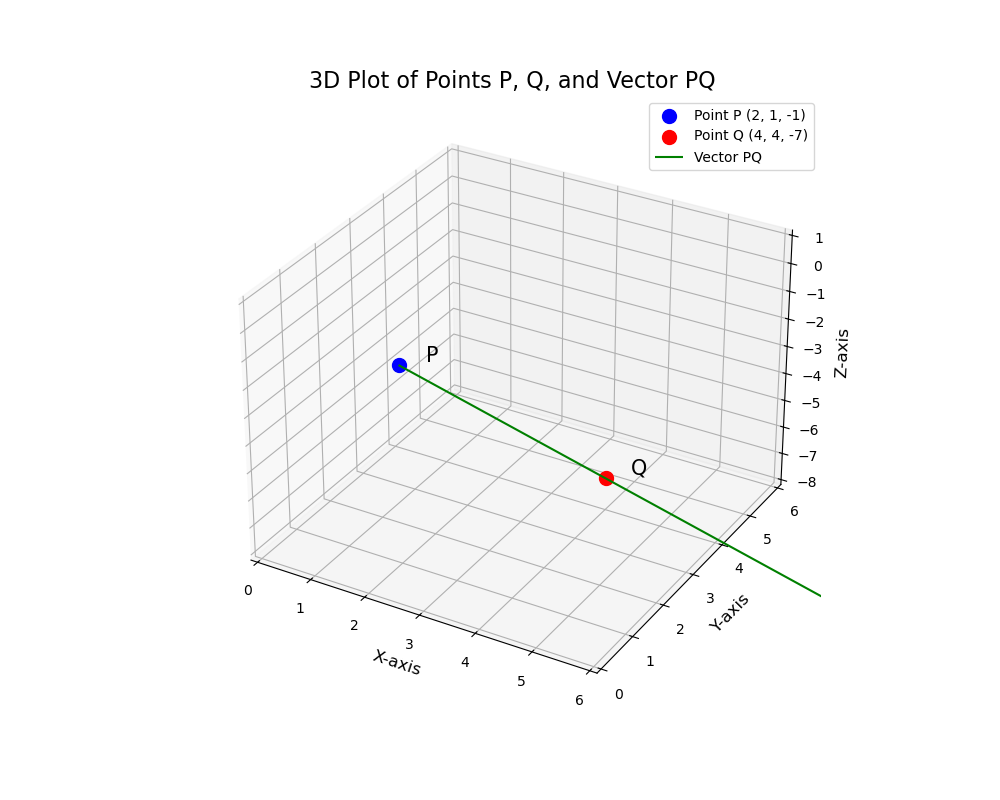
\includegraphics[width=\columnwidth, height=0.8\textheight, keepaspectratio]{figs/fig1.png}     
\end{frame}


\end{document}
